\documentclass{article}

%package setup
\usepackage{graphicx}
\usepackage{amsmath}
\usepackage{fancyhdr}
\usepackage[margin=1in]{geometry}
\usepackage{comment}
\usepackage{placeins}
\usepackage{parskip}
\usepackage{subcaption}
\usepackage{appendix}
\usepackage{soul}
\usepackage{comment}
\usepackage[hidelinks]{hyperref}
\usepackage{matlab-prettifier}
\usepackage{minted}
\usepackage{enumitem}
\usepackage{float}
\usepackage{textcomp, gensymb}
\usepackage{caption}


\pagestyle{fancy}
\fancyhf{} % Clear header/footer settings
\rhead{\thepage} % Page number on the right in the header
\lhead{ASE375 Lab Report 7} % Your lab report title on the left

\begin{document}

\begin{titlepage}
  \centering
  
\includegraphics[width=10cm]{ase-logo-formal.png}  % Adjust the width as needed
  \vspace{1cm}  % Add some vertical space
 
  \Large \textbf{ASE 375 Electromechanical Systems}\\
  \large \textbf{Section 14115}\\
  \vspace{0.5cm}
  \textbf{Monday: 3:00 - 6:00 pm}\\
 
  \vspace{1cm}
 
  \hrule
  \vspace{0.5cm}
 
  \Huge \textbf{Report 7:\\
    Shake Testing}\\
  \Huge \textbf{}\\
 
  \vspace{0.5cm}
  \hrule
 
  \vspace{1cm}
 
  \normalsize \textbf{Andrew Doty, Andres Suniaga, Dennis Hom}\\
  \normalsize \textbf{Due Date: 04/01/2024}
 
\end{titlepage}
\newpage

\tableofcontents
\thispagestyle{empty}
\newpage

\section{Introduction}
In this experiment we analyze the frequency response of a scaled-down wing model using a load cell, MEMS accelerometer, and electromagnetic shaker. The goal of this lab is to learn how a load cell, electromagnetic shaker, and instrumentation amplifier operate by performing a shake test on the scaled-down wing.
\vspace{2.5mm}

The shaker will vibrate the scaled wing model at certain frequencies and the load cell will be measuring the force while the accelerometer will be measuring the motion of the oscillation. From this we will obtain a frequency response function for the wing. This will provide useful information of the wing's structural properties.

\section{Equipment}
Measurement devices and hardware used in this lab include:
\begin{itemize}

\item Built-Up Wing Model: 
\vspace{1mm}

Scaled-down wing model used for shake testing. 

\begin{figure}[H]
    \centering
    \frame{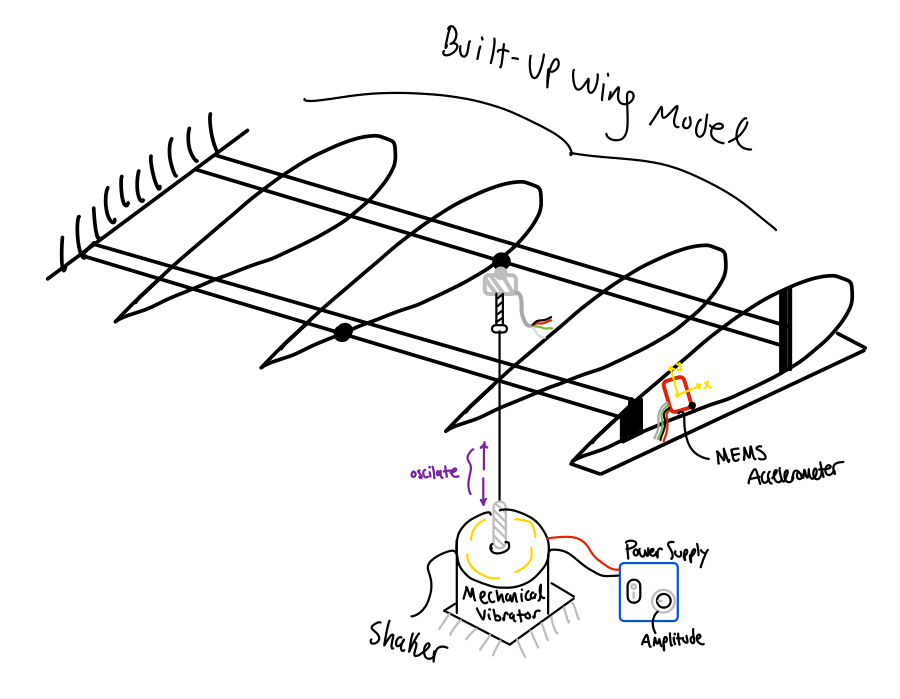
\includegraphics[width = 0.75\textwidth]{lab7/lab7images/wingmodellab7.png}}
    \caption{Built-Up Wing Model Setup, for Part 2 of this Experiment}
    \label{fig:wingsetup}
\end{figure}
\vspace{2.5mm}

\item Strain Gage Load Cell \hyperlink{datasheets}{[5]}:
\vspace{1mm}

Sensor that measures force as an electrical output. Within the load cell there are strain gages set up in a Wheatstone bridge configuration making the load cell's operating principle the variable resistance caused by application of force or deformation which is then measured as an electric signal. The load cell is calibrated in the first part of the lab as shown in Figure \ref{fig:part1} and then placed on a rod atop the shaker to attach to the wing as shown in Figure \ref{fig:wingsetup}.
\vspace{2.5mm}

\item 'Rare Earth' Magnets:
\vspace{1mm}

Small Magnets used for secure placement of load cell under the wing platform.
\vspace{2.5mm}

\item Brass Slotted Weights with hanger and L-bracket:
\vspace{1mm}

L-bracket used for placement of load cell on beam. Weights hanged on L-bracket to calibrate the load cell as shown below:

\begin{figure}[H]
    \centering
    \frame{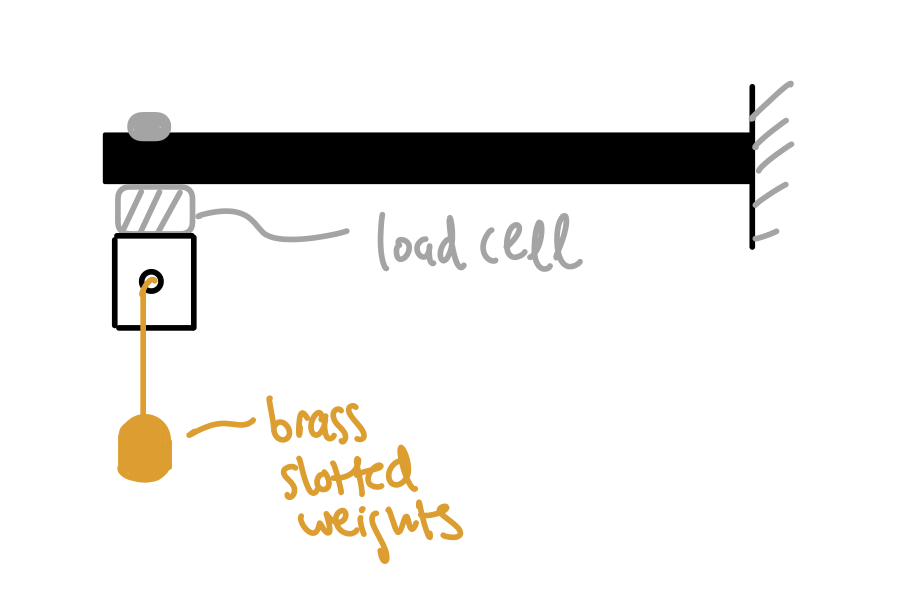
\includegraphics[width = 0.5\textwidth]{lab7/lab7images/loadcellcalib.png}}
    \caption{Placement for Calibration of the Load Cell, for Part 1 of this Experiment}
    \label{fig:part1}
\end{figure}
\vspace{2.5mm}

\item MEMS Accelerometer (ADXL335) \hyperlink{datasheets}{[2]}
\vspace{1mm}

The ADXL335 is a small 3-Axis MEMS Accelerometer which operates based on differential capacitance. An applied force or acceleration will change the capacitance within the MEMS accelerometer. In this experiment, the MEMS accelerometer is placed as shown in Figure \ref{fig:wingsetup}, using only the Y-axis for our experiment. Operational Voltage = $3.3\text{V}$
\vspace{2.5mm}

\item Mechanical Wave Driver \hyperlink{datasheets}{[4]}: 
\vspace{1mm}

Electromagnetic shaker with driver arm capable of oscillating/vibrating at variable amplitudes and any frequency between $0.1\; \text{Hz}$ to $5\; \text{kHz}$. In this experiment it is used to shake the wing model as shown in Figure \ref{fig:wingsetup}. 
\vspace{2.5mm}

\item DAQ, NI-9215 Voltage Input Module \hyperlink{datasheets}{[1]}, NI-9263 Analog Output Module \hyperlink{datasheets}{[6]},  and LabVIEW:
\vspace{1mm}

Data Acquisition System used to process sample measurements into digital data for the computer to read.\\[5pt]
NI-9215 is an analog input module used to measure the output voltage signals of sensors and send it through the DAQ system. The NI-9215 module will measure the output of the instrumentation amplifier \hyperlink{datasheets}{[3]}.\\[5pt]
The NI-9263 output module will connect to the mechanical wave driver to supply it with sinusoidal waves.\\[5pt]
LabVIEW used to model these output voltages read from the DAQ of the accelerometer and load cell measurements. 

\item Solderless Breadboard, Jumper Wires, and AD623 Instumentation Amplifier \hyperlink{datasheets}{[3]} : 
\vspace{1mm}

Used to make connections to the input analog modules and to construct circuits. In this lab we connect the accelerometer inputs to the breadboard for power, ground, and signal for the measurement axis. We also make a circuit for the load cell as shown below:

\begin{figure}[H]
    \centering
    \frame{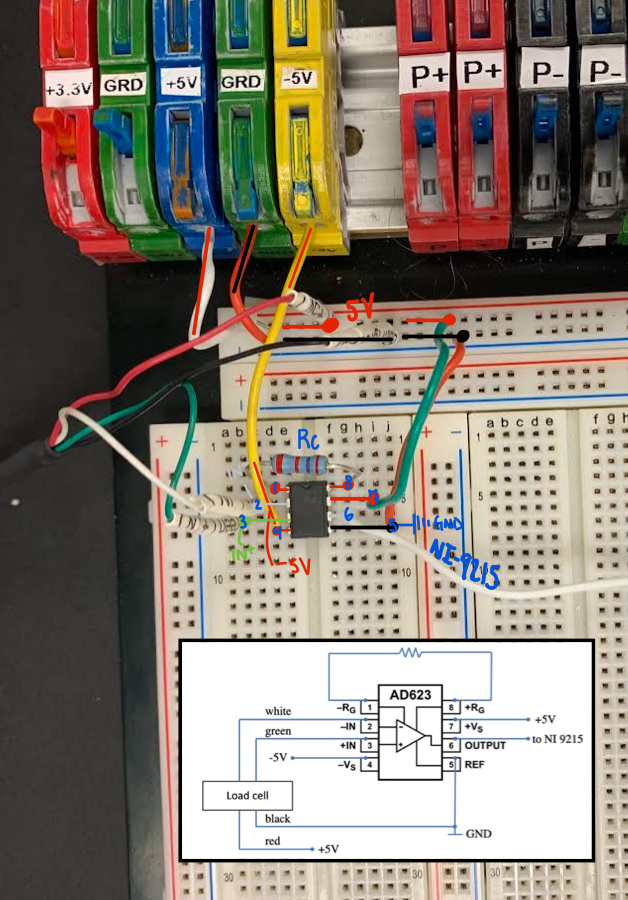
\includegraphics[width=0.75\textwidth]{lab7/lab7images/lab7circuitloadcell.jpg}}
    \caption{Load Cell Amplifier Circuit}
    \label{fig:ampcircuit}
\end{figure}

\end{itemize}

\section{Procedure}
\subsection{Load Cell Calibration}
Before beginning the calibration, ensure the block diagram to gather the data on LabVIEW is setup as shown in the example below:
\begin{figure}[H]
    \centering
    \frame{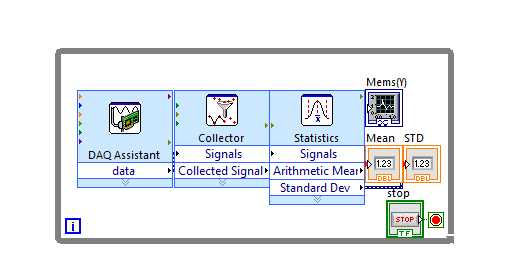
\includegraphics[width=0.75\textwidth]{lab7/lab7images/lab7blockdiagram1.PNG}}
    \caption{LabVIEW Block Diagram Setup Example}
    \label{fig:labview1}
\end{figure}

\begin{itemize}
    \item (DAQ) $\text{Data}\rightarrow \text{Signals}$ (Collector),
    \item (Collector) $\text{Collected Signals}\rightarrow \text{Signals}$ (Statistics),
    \item (Collector) $\text{Collected Signals}\rightarrow \text{Waveform Graph}$,
    \item  $\text{Arithmetic Mean}\rightarrow \text{Mean}$,
    \item  $\text{Standard Deviation}\rightarrow \text{STD}$.
\end{itemize}

This LabVIEW setup will plot the load cell compression and expansion as an electrical output over time as well as calculate the average voltage, $V_{\text{OUT}}$, and standard deviation. These are the values we need to mark down for calibration.
\vspace{1mm}

NOTE: Disregard "Mems(Y)" name over the waveform plot. Rename as "Load Cell".
\vspace{5mm}

Calibrating the load cell:

\begin{enumerate}
    \item First, with the appropriate screws and L-bracket, screw in the top of the load cell to a beam with the L-bracket screwed just underneath the load cell as shown in Figure \ref{fig:part1}. Weights will be hung on the L-bracket to calibrate the load cell.
    \item Measure the gain setting resistor, $R_{G}$ as shown in Figure \ref{fig:ampcircuit}.\\
    NOTE: This step can be done before or after calibrating of the load cell.
    \item Run the LabVIEW model. Load sequence of weights (in grams) to hang on the L-bracket,
    \begin{center}
    $\textbf{w} = \left[0,\, 50,\, 70,\, 90,\, 110,\, 130,\, 150,\, 170,\, 190,\, 210,\, 230,\, 250,\, 270\right]$
    \end{center}
    Zero means no weight on the bracket and 50 grams is the weight of the hangar by itself. 
    \item Mark down measurements of the average electrical output (mean) and the standard deviation.
    \item This data can be found in \hyperlink{datapro}{Data Processing}
\end{enumerate}

\subsection{Shake Testing}
\textbf{Block Diagram:} Open "sineswept.vi" for LabVIEW. This will allow the software to send sinusoidal waves through a range of frequencies from $5\, \text{Hz}$ to $100\, \text{Hz}$ to the shaker, which we will use for this experiment. Use $1\, \text{kHz}$ sampling frequency.
\vspace{5mm}

Shake Test:
\begin{enumerate}
    \item Connect the MEMS accelerometer and load cell to the circuit board (amp circuit for load cell shown in Figure \ref{fig:ampcircuit}) and respective NI-9215 input modules. Ensure Shaker is connected to the NI-9263 output module to receive sinusoidal waves of different frequencies. Setup the wing model for shake testing as shown in Figure \ref{fig:wingsetup}.
    \item Issues to prevent before beginning shake test:
    \begin{itemize}
        \item Load Cell Slippage off the wing model
        \item Bent Rod joining the load cell and mechanical wave driver
        \item Slanted or Loose Accelerometer
    \end{itemize}
    \item Adjust the amplitude for the wave driver as needed. For this experiment, our amplitude was placed on the lower end of the knob values.
    \item Perform shake test by running the LabVIEW Sine Swept model. The wing will start shaking and frequency will increase until $100\, \text{Hz}$ is reached.
    \item Restart shake test if load cell slips off or accelerometer comes loose. 
    \item Once the shake test concludes, save the data which will be written to a file.
    \item Next up is \hyperlink{datapro}{Data Processing} to find the Frequency Response function of the wing.
\end{enumerate}

\hypertarget{datapro}{}
\section{Data Processing}
\subsection{Variables and Equations}  

Gain of the AD623 Instrumentation Amplifier:
\begin{equation}
    G = 1 + \dfrac{100\, \text{k}\Omega}{R_{G}}
\end{equation}

Variables:
\begin{itemize}
    \item \(R_{G}\): Resistance of Gain setting resistor
\end{itemize}
\vspace{5mm}

Differential Voltage, Output Voltage (read by DAQ) is amplified by Gain $G$:
\begin{equation}
    V_{\text{OUT}} = GV_{0}
\end{equation}

Variables:
\begin{itemize}
    \item \(V_{\text{OUT}}\): Output voltage read by DAQ
    \item \(V_{0}\): Input voltage going into Instrumentation Amp
\end{itemize}
\vspace{5mm}

Harmonic Motion Equations:
\begin{equation}
    x(t) = A\sin{(\omega t)}
\end{equation}
\begin{equation}
    \ddot{x}(t) = -A\omega^{2} \sin{(\omega t)}
\end{equation}

With these harmonic motion equations we can make the estimation:
\begin{center}
    \(|x| = A\), \hspace{10mm} \(|\ddot{x}| = A\omega^{2}\), \hspace{10mm} \(\implies |x| = \dfrac{|\ddot{x}|}{\omega^{2}}\)
\end{center}

Variables:
\begin{itemize}
    \item \(x(t)\): Displacement as a function of time
    \item \(\ddot{x}(t)\): Acceleration as a function of time
    \item \(A\): Amplitude
    \item \(\omega\): Frequency
\end{itemize}
\vspace{5mm}

    
\section{Results and Analysis}


\section{Conclusion}


\newpage
\thispagestyle{empty}  % Clear header/footer
\begin{center}
	\vspace*{\fill}
	{\Huge Appendix}
	\vspace*{\fill}
\end{center}

% Start appendices
\newpage
\begin{appendices}
\pagestyle{fancy}
\renewcommand{\thefigure}{A\arabic{figure}}
\setcounter{figure}{0}

% \section*{t-Distribution Tables}
% \hypertarget{1}{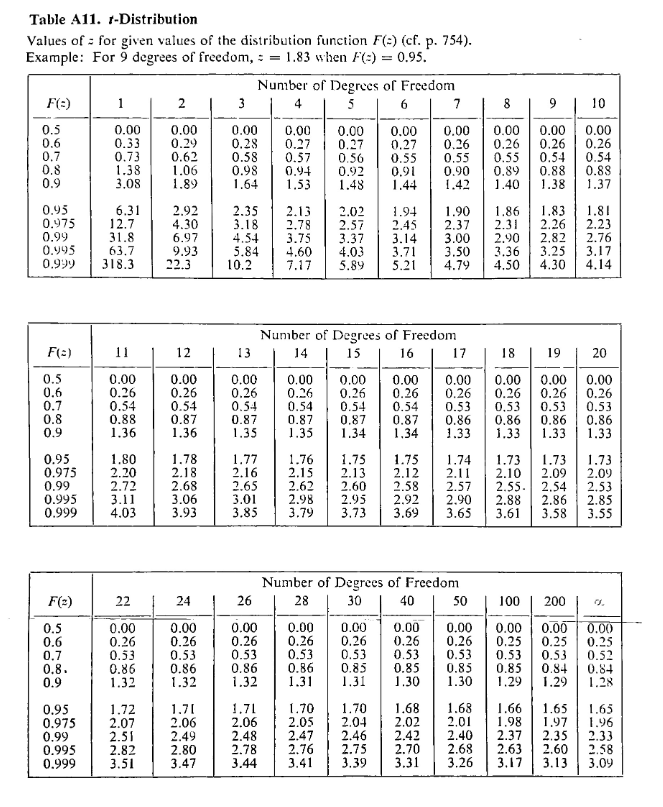
\includegraphics[width=0.95\textwidth]{t_distribution_Table_lecture3.png}}

%Add other appendix items here

\pagebreak

\hypertarget{datasheets}{}
\section{Datasheets}
\begin{enumerate}[label = {[\arabic*]}]
\item \textbf{NI-9215 Datasheet:}\\[2pt] \url{https://www.amc-systeme.de/files/pdf/ni-9215-amc.pdf}

\item \textbf{ADXL335 Accelerometer Datasheet:}\\[2pt] \url{https://www.analog.com/media/en/technical-documentation/data-sheets/adxl335.pdf}

\item \textbf{AD623 Instrumentation Amplifier Datasheet:}\\[2pt]
\url{https://www.analog.com/media/en/technical-documentation/data-sheets/ad623.pdf}

\item \textbf{Mechanical Wave Driver (SF-9324) Specs:}\\[2pt]
\url{https://cdn.pasco.com/product_document/Mechanical-Wave-Driver-Manual-SF-9324.pdf}

\item \textbf{Miniature Low-Profile Tension Link Load Cell Specs:}\\[2pt]
\url{https://br.omega.com/omegaFiles/pressure/pdf/LCM703.pdf}

\item \textbf{NI-9263 Datasheet:}\\[2pt] \url{https://www.ni.com/docs/en-US/bundle/ni-9263-specs/page/specs.html}

\end{enumerate}

\end{appendices}

\end{document}
